\subsection{Network split}

\begin{figure}[htb!]
  \centering
    \subfloat[]{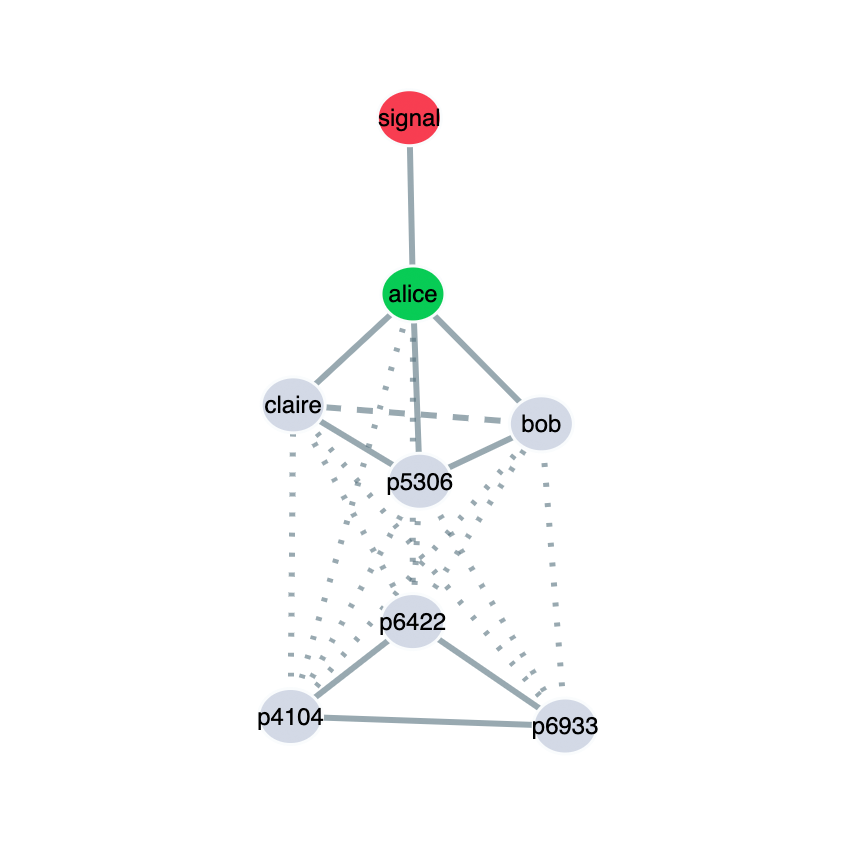
\includegraphics[width=0.25\textwidth]{graphics/analysis/mini-scenarios/network-split/1.png} \label{fig:filmstrips-network-split-a}}
    \subfloat[]{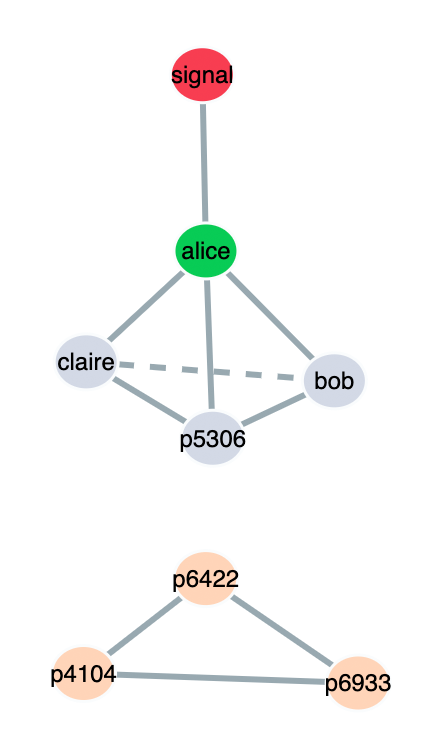
\includegraphics[width=0.25\textwidth]{graphics/analysis/mini-scenarios/network-split/2.png} \label{fig:filmstrips-network-split-b}}
	\subfloat[]{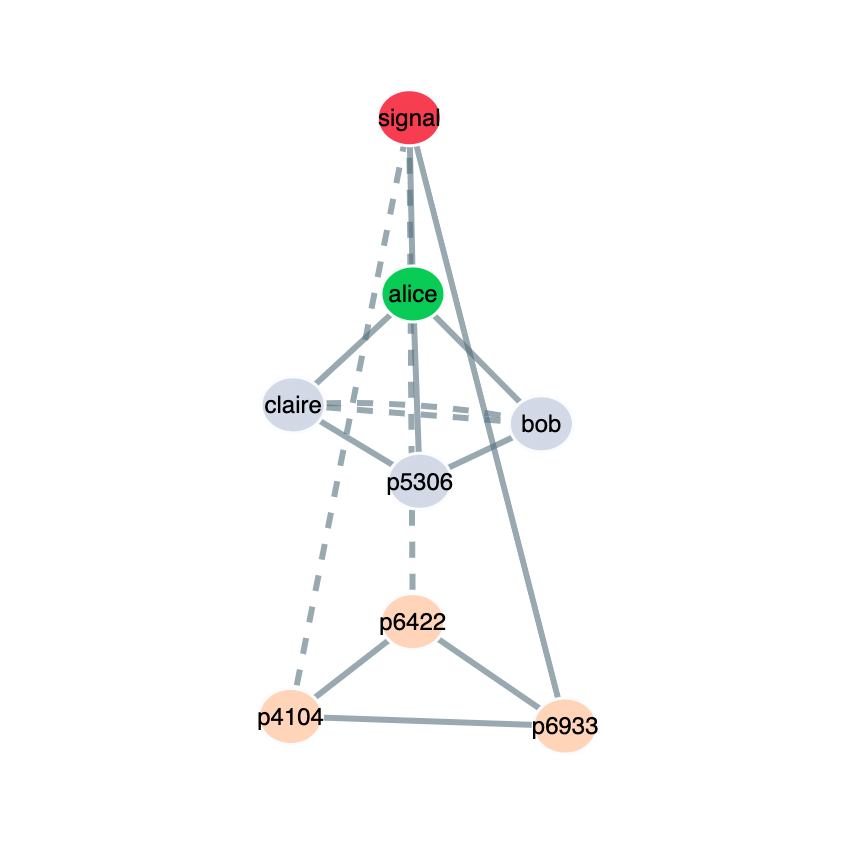
\includegraphics[width=0.25\textwidth]{graphics/analysis/mini-scenarios/network-split/3.png} \label{fig:filmstrips-network-split-c}}
	\subfloat[]{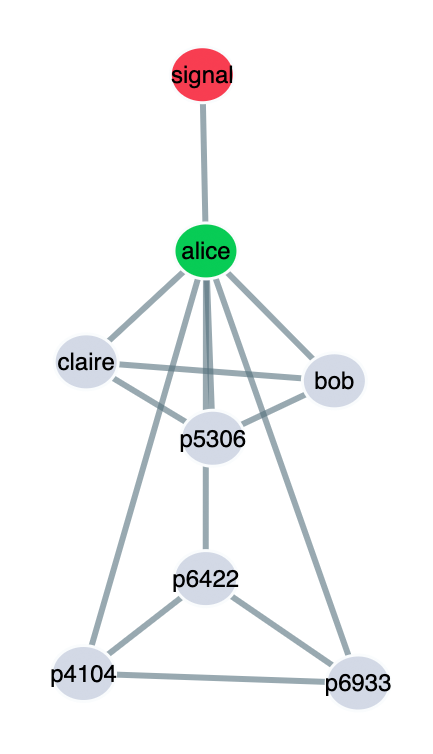
\includegraphics[width=0.25\textwidth]{graphics/analysis/mini-scenarios/network-split/4.png} \label{fig:filmstrips-network-split-d}}
	\caption{Group of nodes looses contact to main network}
\label{fig:filmstrips-network-split}
\end{figure}

Mitosis tries to prevent network splits through the \textit{Router-Gravity} metric, but it can not prevent that a group or a single peer eventually diverges from the main network. 

\vref{fig:filmstrips-network-split-a} shows a scenario where a split was enforced by closing connections with the visualisation tool. As the nodes do not have global knowledge of the network they do not know that they have lost the connection to the main network immediately.

Each \lstinline|RemotePeer| in the \lstinline|PeerTable| of a node has an expiration date based on its LastSeen timestamp. This is updated every time a message has been received. When LastSeen exceeds a hard defined threshold, the peer is removed from the PeerTable.

The peer with the role \router, \alice, is constantly sending \routerAlive messages. Thus, the last seen of \alice is always updated if any path from \alice to the peer exist. 
In \vref{fig:filmstrips-network-split-b} the LastSeen has exceeded the threshold and therefore the router peer \alice is removed from the PeerTable. Mitosis specifies that, when a peer does not have any RemotePeer in its PeerTable with the role \router, it is degraded to the role \newbie.

A peer with the role \peer is contacting the \signal peer to re-enter the network (\vref{fig:filmstrips-network-split-c}). As \alice has available connections, the negotiation offer is accepted, thus a connection is established. The \routerAlive message is funneled to through has re-entered the network, thus all peers know that they have been absorbed into the main network (\vref{fig:filmstrips-network-split-d}).